%%%%%%%%%%%%%%%%%%%%%%%%%%%%%%%%%%%%%%%%%%%%%%%%%%%%%%%%%%%%%%%%%%%%%%%%
\chapter{Diseño}
\label{ch:diseno}
 
  El análisis de los requisitos presentados en el capítulo \ref{ch:requisitos} dará como resultado la arquitectura de la aplicación. Para llevar a cabo su desarrollo, hemos tenido en cuenta la arquitectura del dispositivo y las herramientas adjuntas para el desarrollo de aplicaciones. Todas las decisiones tomadas en la construcción de la arquitectura de la aplicación se han basado en los límites o restricciones impuestas por el uso de la arquitectura de Apple y los límites impuestos en el uso del API de Betfair. Para comprender mejor el diseño de la aplicación expondremos brevemente la arquitectura impuesta por Apple en el iPhone y la tecnología en la que se basa el API que ofrece Betfair para el uso de sus servicios.

\section{API de iOS: Cocoa Touch}
 La arquitectura del terminal móvil se basa en su sistema operativo \emph{iOS} de Apple. Este sistema operativo, a grandes rasgos, es un subconjunto del sistema operativo que llevan los ordenadores personales de Apple. Esta decisión favorece el desarrollo de aplicaciones para sus plataformas. Simplifica la tarea a los desarrolladores de aplicaciones de ordenadores de sobremesa de Apple de programar aplicaciones móviles sin necesidad de aprender un lenguaje o arquitectura totalmente nueva.
 
 %\fxnote{La introducción de gráficos o figuras puede hacerse de dos
  % formas: o la ``empotras'' directamente como he hecho yo con la
   %figura de las capas del OS o la metes en un entorno ``figure'' y la
   %referencias con un ``ref'' como he hecho con la figura \ref{fig:API
    % Betfair}, lo que creas más conveniente}

\noindent
La siguiente figura muestra la estructura en forma de capas en las que se compone el sistema operativo \emph{iOS}:

%\begin{center}
%  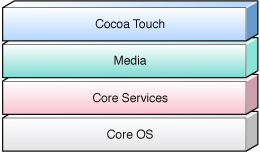
\includegraphics[width=0.5\textwidth]{./images/overview_systemlayers.jpg}
%\end{center}

\begin{figure} [h]
  \centering
    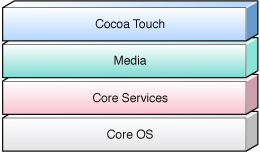
\includegraphics[width=0.6\textwidth]{./images/overview_systemlayers.jpg}
  \caption{Capas del \emph{iOS}}
  \label{fig:Capas-del-iOS}
\end{figure}

En la parte baja del sistema se encuentran las capas encargadas de los
servicios fundamentales que permiten la ejecución de las aplicaciones,
y en las superiores contienen las capas sobre los servicios multimedia
y de las más altas tecnologías.
 

A continuación expondremos una breve descripción de cada capa:

%\fxnote{He cambiado el entorno ``itemize'' a ``description'' para que
 % veas como queda, si te gusta lo mantienes, si no lo cambias. También
 % he modificado la indentación en el código fuente de latex para que
 % veas que se pueden meter cambios de linea sin probleamas (dos
 % cambios de linea consecutivos = nuevo párrafo).}

\begin{description}
\item[Core OS.]  Es la capa que contiene el núcleo de
  sistema (\emph{kernel}) %\fxnote{Recuerda, inglés enfatizado, al
   % menos en la primera aparición, encárgate tú del resto.},
  , los controladores para dispositivos internos y las interfaces básicas del sistema
  operativo. El kernel es el responsable de todos los aspectos
  relacionados con el sistema operativo. Es el encargado de gestionar
  la memoria virtual, \emph{threads} (procesos ligeros), sistema de ficheros,
  red y procesos de comunicación. Los controladores son los encargados
  de proporcionar la interfaz entre el \emph{hardware} y los \emph{frameworks} de
  las capas superiores.
\item[Core Services.] Es la capa responsable de proporcionar los
  servicios básicos del sistema a las aplicaciones para su uso. En
  ella encontramos el acceso a la agenda del dispositivo, la gestión
  de estructura de datos, la gestión de las interfaces de red, la
  gestión de la localización del dispositivo, la gestión de la seguridad
  del sistema y el soporte para bases de datos SQL y XML.
\item[Media.] Es la capa encargada de dar soporte a las
  tecnologías de gráficos y al audio y video para proporcionar al usuario
  los medios multimedia vistos en un dispositivo móvil.
\item[Cocoa Touch.]  Es una de las capas más importantes del iOS
  para un desarrollador de aplicacionesmóviles. Se encarga de las interacciones del usuario con la interfaz táctil del dispositivo. 
 \end{description}
  
  Esta última capa es la que diferencia la plataforma móvil de la plataforma PC en los entornos de Apple. Una vez visto lo esencial del sistema operativo \emph{iOS}, Apple nos proporciona en su API un conjunto de \emph{frameworks}\footnote{Un framework es una estructura de soporte definida, en la cual otro proyecto de software puede ser organizado y desarrollado.} para poder acceder a las capas vistas anteriormente. Los más importantes son:  

 \begin{description}
 	\item [UIKit.] Contiene todas las clases necesarias para la programación de la interfaz de usuario de las aplicaciones así como el acceso a las principales tecnologías hardware 
	 propias del dispositivo  móvil. Es la más importante de todos los emph{framework} ya que haciendo uso de ella crearemos la interfaz de usuario de nuestra aplicación:
		 \begin{itemize}
		  	\item soporte para la creación de gráficos y ventanas del sistema.
			\item soporte para la gestión de eventos \emph{multitouch} y eventos realizados al pulsar la pantalla con más de un dedo.
			 \item soporte para la creación de contenido tanto de texto como de web.
 			\item soporte para la creación de controles y objetos del sistema.
 			\item soporte para copiar, cortar y pegar.
 			\item soporte para la accesibilidad de aplicaciones.
 			\item soporte para el acceso a las capacidades hardware del dispositivo: batería, cámara, acelerómetros, sensor de proximidad \ldots 
 		\end{itemize}
 	 \item [Foundation.] Es un \emph{framework} heredado de la plataforma OS X. Provee el soporte para las siguientes funcionalidades: 
 		\begin{itemize}
			\item colecciones de datos (arrays, sets \ldots)
			\item gestión del tiempo y fechas.
			\item gestión de las preferencias del dispositivo.
			\item gestión de URLs.
			\item internacionalización del dispositivo.
		\end{itemize}
	\item [Address Book UI.] Una de las partes más usadas en un dispositivo móvil es la agenda de contactos. Nos proporciona las herramientas necesarias para acceder a los contactos del dispositivo: crear, modificar, eliminar \dots
	\item [Message UI.] Proporciona el soporte necesario para componer y gestionar mensajes de correo electrónico o \emph{SMS} en nuestras aplicaciones.
	\item [Map kit.]  Esta interfaz proporciona la creación de una vista de un mapa geográfico escalable con posibilidad de incrustar en él información detallada. Un típico ejemplo es la localización en un mapa de un restaurante.
	\item [Push Notification Service.] Proporciona un camino para notificar a los usuarios que una aplicación tiene nueva información relevante. El sistema notifica al usuario la información incluso si la aplicación no está en ejecución.

\end{description}

 Para poder desarrollar aplicaciones para dispositivos iOS, Apple pone a disposición de forma gratuita un conjunto de herramientas de desarrollo (SDK) que se encuentra disponible en su portal web. 

\section{Arquitectura del API de Betfair}

	Los servicios web que nos proporciona el API de Betfair están diseñados bajo un protocolo \emph{SOAP}\footnote{Simple Object Access Protocol}. \emph{SOAP} es un protocolo estándar que define cómo dos objetos en diferentes procesos pueden comunicarse por medio de intercambio de mensajes, en este caso codificados en \emph{XML}\footnote{Extensible Markup Language, es un metalenguaje extensible de etiquetas desarrollado por el World Wide Web Consortium (W3C).}. A continuación explicaremos qué son y cómo funcionan los servicios web para más adelante comprender las decisiones tomadas en la arquitectura de la aplicación.
	%\fixme{Esto hay que solucionarlo mediante una referencia bibliográfica utilizando bibtex, pregunta si no sabes cómo y lo vemos juntos.} 

%\fixme{Creo que se hace fundamental explicar en qué consiste todo este asunto del WSDL, cómo se usa (probablemente hay varios ``workflows'' posibles), un par de ejemplos pueden ser determinantes para entender la filosofía. En estos %momentos, como lector, estoy más interesado en que me cuentes cómo se materializa ese API que en ningún otra cosa. También puedes dar el ejemplo un poco más adelante y avisar al lector. Puedes utilizar subsections para organizar %bien la exposición.}

\subsection{Servicios web}

         Un servicio web es una interfaz de software que describe un conjunto de servicios u operaciones a las cuales se puede acceder por la red. El acceso a dichos servicios se realiza a través de intercambios de mensajes estandarizados. Para su comunicación usa protocolos basados en el lenguaje \emph{XML} con el objetivo de describir una operación para ejecutar o datos para intercambiar con otro servicio web.  
 
\begin{figure} [h]
  \centering
    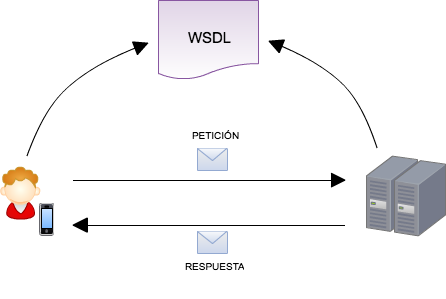
\includegraphics[width=0.6\textwidth]{./images/webservice.png}
  \caption{Funcionamiento servicios web}
  \label{fig:servicioweb}
\end{figure}
         
         Según el ejemplo de la figura \ref{fig:servicioweb}, un cliente, a través de una aplicación, realiza una petición de uso de un servicio web a través de un mensaje que ofrece un proveedor a través de Internet. El proveedor responderá a la petición con la información requerida en un mensaje con destino el cliente. En todo este proceso intervienen una serie de tecnologías que hacen posible esta circulación de información. Por un lado, estaría \emph{SOAP}. Se trata de un protocolo basado en \emph{XML}, que permite la interacción entre varios dispositivos y que tiene la capacidad de transmitir información compleja. Los datos son transmitidos a través de HTTP\footnote{Hypertext Transfer Protocol}, es el método más común de intercambio de información en la web, el método mediante el cual se transfieren las páginas web a un ordenador. 
          Por otro lado, \emph{WSDL}\footnote{Web Services Description Language} permite que un servicio y un cliente establezcan un acuerdo en lo que se refiere a los detalles de transporte de mensajes y su contenido, a través de un documento procesable por dispositivos. \emph{WSDL} representa una especie de contrato entre el proveedor y el que solicita. WSDL especifica la sintaxis y los mecanismos de intercambio de mensajes.
                    
 \subsection{Servicios web de Betfair }
 	El API de Betfair está disponible a partir de un fichero en formato \emph{WSDL} en el portal de desarrolladores de Betfair. Dicho formato describe la interfaz para todos los servicios web disponibles de Betfair. En el capítulo \ref{ch:implemetacion} describiremos cómo hemos hecho uso de este fichero para construir las llamadas al servidor y consumir dichos servicios de Betfair.

 Los servicios web proporcionados por el API de Betfair se dividen en dos conjuntos: 
          
\begin{itemize}
	\item \emph{Global}: contiene todas las llamadas referentes a los servicios básicos de Betfair, tales como el inicio de sesión, la administración de tu cuenta Betfair, tus fondos y las llamadas para navegar por los diferentes eventos disponibles en el portal de apuestas. 
	\item \emph{Exchange}: contiene las llamadas a los servicios relacionados con las apuestas, es decir, apostar por un evento, descripción de los mercados disponibles, actualización o cancelación de las apuestas ya realizadas, historial de todas nuestra apuestas\ldots 
\end{itemize}

  Para cada conjunto existen dos formas de acceso al API:
\begin{description}
	\item [Free Access API.]  Con este acceso tendremos disponibles los servicios básicos del portal y las herramientas suficientes para poder apostar por los eventos disponibles. Gratuito pero no contiene todos los servicios que proporciona Betfair.
	\item [Full Access API.] Acceso de pago donde están disponibles todos los servicios exclusivos del portal tales como la gestión de acceso a nuestro medio de pago de nuestra cuenta de usuario\ldots Se gestiona a partir de una cuota anual y no existen límites en las llamadas a los servicios del API.
\end{description}

Resaltar en este apartado que dado que nuestra aplicación no soporta la plataforma \emph{WSDL}, hubo que implementar cada llamada a los servicios de Betfair bajo la tecnología de Apple y su posterior serialización para el tratamiento de datos de la aplicación. Por cada llamada descrita en el archivo de definición de servicios hemos tenido que implementar la estructura de la comunicación mediante mensajes \emph{XML}, uno de petición y otro de respuesta con un \emph{parser} asociado que traduzca dichos mensajes. En el capítulo \ref{ch:implemetacion} veremos con más detalle la adaptación de \emph{WSDL} a la plataforma \emph{iOS}.

\subsection{Servicios básicos necesarios}

    Los servicios básicos que hemos usado para el cumplimiento de los requisitos de la aplicación han sido:

\begin{itemize}
	\item \lstinline{Login}: 
		llamada para poder usar los servicios web de Betfair. 
	\item \lstinline{GetActiveEventTypes}: 
		con esta llamada obtenemos todos los eventos deportivos actualmente en marcha por los que se puede apostar.
	\item  \lstinline{GetAllMarkets}:
		con esta llamada obtenemos todos los mercados referentes a un evento.
	\item  \lstinline{GetCurrentsBets}:
		llamada por la cual obtenemos todas las apuestas activas que hemos realizado.
	\item  \lstinline{GetMarketPrices}:
		obtenemos los precios (back y lay) actuales por un evento determinado.
	\item  \lstinline{GetMarket}:
		esta llamada nos devuelve todos los datos referentes a un mercado.
	\item  \lstinline{PlaceBets}:
		con esta llamada enviamos una apuesta a Betfair.
	\item  \lstinline{ViewProfile}: 
		esta llamada nos devuelve los datos de perfil de usuario.
	\item  \lstinline{RetrieveLIMBMessage}:
		 con esta llamada obtenemos los mensajes del sistema pendientes de acción por parte del usuario.
\end{itemize}

\section{Arquitectura de la aplicación}

%\fixme{Averiguar a qué modelo MVC más se parece lo que has hecho y hablar de él a un nivel similar al que lo hace Fowler en http://martinfowler.com/eaaDev/uiArchs.html,  http://aspiringcraftsman.com/2007/08/25/interactive-application-architecture/ o http://www.codeproject.com/Articles/42830/Model-View-Controller-Model-View-Presenter-and-Mod}

 Para el diseño de la arquitectura nos hemos basado en el patrón de diseño ``Modelo Vista Controlador (MVC)'', exactamente Modelo Vista Controlador de Smalltalk. Dicho patrón es muy utilizado en la programación orientada a objetos, donde los objetos del modelo representan los datos de la aplicación y son persistentes. Fundamentalmente consiste en separar los datos de una aplicación, la interfaz de usuario, y la lógica de control en tres componentes distintos:

 \begin{description}
 	\item [Modelo.] Es la representación de toda la información con la cual el sistema trabajará. El modelo es independiente de cualquier representación o vista.
	\item [Vista.] Se encarga de presentar el modelo en un formato adecuado para interactuar, normalmente mediante una interfaz de usuario.
	\item [Controlador.] Se encarga de responder a eventos. Esto implica cambios en el modelo y en la vista.
\end{description}
 
  La razón del uso de este patrón se debe a dos cuestiones fundamentales:
\begin{itemize}
	\item La facilidad entre la comunicación del modelo de datos y entre la interfaz. Cualquier cambio en la interfaz de usuario no afecta al resto del modelo, por lo que se gana en facilidad a la hora de seguir desarrollando la solución en el futuro.
	\item Apple, en el uso de las herramientas de desarrollo del SDK, recomienda el uso de dicho patrón para la creación de la interfaz de usuario de la aplicación. Esta recomendación es debido a la arquitectura interna del \emph{iOS} y a que sus herramientas de desarrollo también están orientadas a esta solución.
	\item La estructura jerárquica de los datos obtenidos a través del API de Betfair. Este patrón nos facilita la representación de los mismos.
\end{itemize}

%\fxnote{MVC es un nombre demasiado genérico y bastante manido, quizás quieras explorar con más profundidad las características exactas del patrón que hayas aplicado: http://www.aspiringcraftsman.com/2007/08/interactive-application-architecture/, http://c2.com/cgi/wiki?MvcIsNotObjectOriented}

\subsection{Núcleo de la aplicación}
	Toda aplicación para \emph{iOS} se desarrolla usando principalmente el \emph{framework} UIKit. UIKit proporciona todo lo necesario para lanzar la aplicación, coordinar los \emph{inputs} del usuario y mostrar el contenido en la pantalla. 
	Desde que el usuario pulsa el icono de la aplicación hasta que esta es ejecutada , el \emph{framework} UIKit gestiona todo lo necesario para lanzar la infraestructura. Toda aplicación recibe principalmente eventos continuamente desde el sistema y debe responder a todos estos eventos. 
	
	El ciclo de una aplicación esta formado por la secuencia de eventos del sistema:  pulsación en la pantalla por parte del usuario, llegada de un mensaje de texto\ldots que ocurren entre la ejecución y la finalización de la aplicación. En \emph{iOS}, el usuario lanza la aplicación pulsando sobre el icono de la misma en la pantalla.  A partir de este momento, UIKit es el encargado de lanzar la interfaz de usuario y de leer los eventos que se produzcan en un bucle hasta que la aplicación sea finalizada bien por el sistema o bien por el usuario. Durante el bucle, UIKit coordina la llegada de eventos a los objetos (el usuario pulsa una parte de la pantalla) y coordinar las respuestas de las mismas, es decir, qué hacer ante la acción del usuario. 
	     
 \begin{figure} [h]
  \centering
    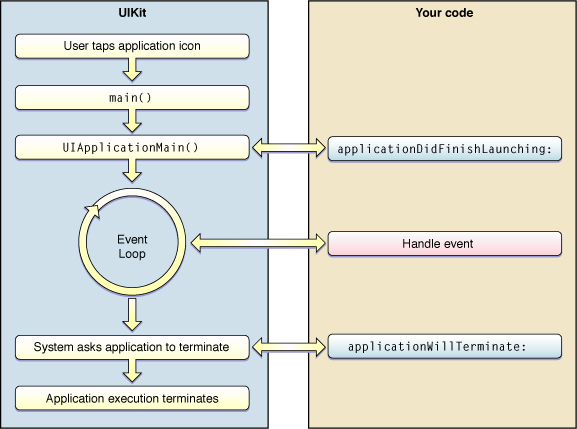
\includegraphics[width=0.8\textwidth]{./images/app_life_cycle.jpg}
  \caption{Ciclo de una aplicación \emph{iOS} }
  \label{fig:iOS-layers}
\end{figure}
     
   La figura \ref{fig:iOS-layers} muestra el ciclo de una aplicación para \emph{iOS}. Tal y como vemos, UIKit se encarga del arranque de la aplicación y de la gestión de eventos. Nuestro código será el encargado de gestionar esos eventos cuando reciba la notificación de que la aplicación ha sido lanzada. También podremos gestionar las accionas oportunas (guardar preferencias o cambios producidos en la aplicación) cuando UIKit nos notifique la finalización de la aplicación.
   
    En \emph{iOS} sólo se finaliza una aplicación por tres motivos:
    \begin{itemize}
	\item El usuario finaliza la misma pulsando el botón \textsf{Home}. 
	\item El sistema recibe una notificación prioritaria que atender, una llamada por ejemplo, y por tanto finaliza la aplicación.
	\item El sistema detecta un comportamiento erróneo de la aplicación y para salvaguardar la estabilidad del sistema finaliza nuestra aplicación.
     \end{itemize}

 \begin{figure} [h]
  \centering
    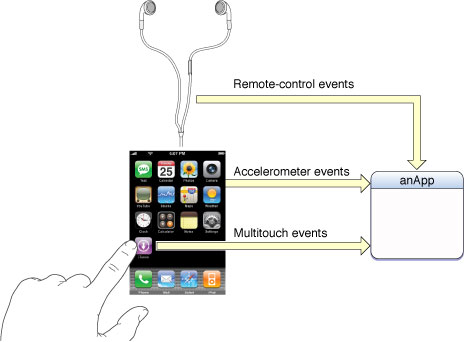
\includegraphics[width=0.8\textwidth]{./images/events_to_app.jpg}
  \caption{Notificaciones del sistema \emph{iOS} }
  \label{fig:iOSnotify}
\end{figure}

 La figura \ref{fig:iOSnotify} muestra un ejemplo de las notificaciones que puede recibir una aplicación por parte del sistema.
 
    Es responsabilidad del desarrollador asociar a cada evento un método adecuado para gestionarlo. Si el desarrollador deja un evento sin asociar, la aplicación simplemente lo ignorará. En nuestra aplicación, gestionamos acciones antes las siguientes notificaciones:
    
\begin{itemize}
	\item \lstinline{didFinishLaunchingWithOptions}: El sistema nos indica que nuestra aplicación ha sido lanzada y tomamos el control a partir de ese momento. 
 	\item \lstinline{applicationWillTerminate}: El sistema nos indica que finalizará nuestra aplicación para salvaguardar la estabilidad del sistema. Básicamente guardaremos el estado de la aplicación.
	\item \lstinline{applicationDidEnterBackground}: El sistema nos indica que nuestra aplicación para a segundo plano. Guardaremos el estado de la aplicación y suspenderemos cualquier acción que este en curso.
\end{itemize} 
    
%\fixme{Dudas que me surgen y que no se si este es el sitio o el momento adecuado para resolverlas. Lo que sí se es que impactan en el diseño: ¿qué eventos llegan al ``Your code''? ¿Qué reglas existen para tratarlos? ¿Se enlazan los eventos a métodos? ¿Se puede modificar ese supuesto ``vector de interrupciones''? ¿Los eventos son independientes de los objetos gráficos? Seguro que contestas a estas preguntas más adelante pero a mi, como lector, me gustaría saber algo más ahora.}    
    
\subsection{Controladores de Vista}	   
 
 Un controlador de vista del SDK proporciona la lógica básica de interfaz de usuario para dibujar las vistas de la aplicación. Definimos como vista de usuario la pantalla que se le presenta en un momento dado. El sistema dispone de varios patrones de interfaces de usuario para ayudar a representar el conjunto de datos hacia el usuario en las aplicaciones dentro de los dispositivos móviles. 
 
  Un controlador de vistas gestiona la vista de nuestra aplicación que aparece entre las barras superiores e inferiores (véase figura \ref{fig:layout-of-views}).
  La vista de la aplicación aparece entre la barra de estado y la barra de navegación si ésta está presente. En una vista de aplicación se muestra una parte de datos y controles que el desarrollador quiere mostrar al usuario en un tiempo determinado. El controlador de la vista simplemente gestiona la presentación de esta vista y la siguiente en aparecer para un patrón de diseño establecido.
 
 \begin{figure} [h]
  \centering
    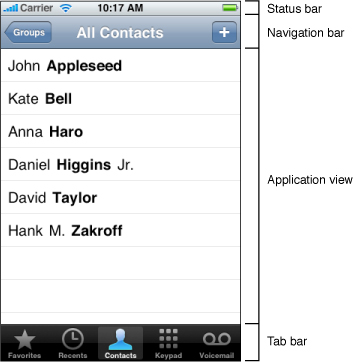
\includegraphics[width=0.8\textwidth]{./images/vc-areas.jpg}
  \caption{Esquema de las vistas }
  \label{fig:layout-of-views}
\end{figure} 
 
 Los controladores de vista nos ahorran código al automatizar la presentación de cada vista al usuario. Es decir, excluyen al desarrollador de tareas tan básicas como la presentación de los objetos en pantalla o la captura de los inputs del usuario. También ayudan al diseño orientado de objetos separando los detalles de la interfaz de usuario de la lógica de la aplicación.
  
 \subsection{Controlador Vista de tablas}	

  Es muy común usar vistas de tabla para mostrar un conjunto de datos de tipo jerárquico para poder recorrerlos.  
  Para ello, disponemos de un controlador específico llamado ``Controlador de vistas de tabla'' que nos proporciona todo lo necesario para su representación y gestión. En nuestra aplicación, tenemos que mostrar el modelo de datos que recogemos de los servidores de Betfair. Éstos están organizados de forma jerárquica, de lo más general a lo más específico. Recordemos que el modelo se basa básicamente en eventos y mercados, y que cada evento puede contener más eventos y mercados. Para poder realizar una apuesta en un partido de fútbol concreto antes hemos tenido que elegir deporte, categoría, país, división y finalmente el partido. La mejor forma de representarlos es mediante una vista de tabla tal y como nos recomiendan las hojas de estilo de Apple.
  
   En la figura \ref{fig:table-view-top} podemos ver un esquema representativo de la información más general. Este caso se podría representar los eventos más altos del modelo de datos de Betfair.
  
 \begin{figure}[h!]
  \centering
    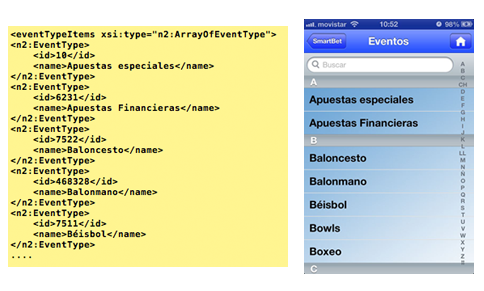
\includegraphics[width=0.8\textwidth]{./images/tabla_top.png}
  \caption{Vista de tabla del top de la jerarquía }
  \label{fig:table-view-top}
\end{figure} 

 En la figura \ref{fig:table-view-middle} nos encontramos una información de tipo jerárquica en la mitad de recorrido. Comparándolo con el modelo de Betfair sería la representación de eventos y mercados en la misma vista. Podemos asociarla al ejemplo de la elección de la división.

\begin{figure}[ht!]
  \centering
    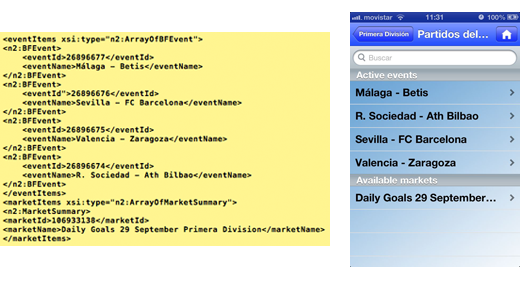
\includegraphics[width=0.8\textwidth]{./images/tabla_middle.png}
  \caption{Vista de tabla de la mitad de la jerarquía}
  \label{fig:table-view-middle}
\end{figure} 

 A continuación representamos el final de nuestro recorrido por el modelo de datos. Como podemos observar en la figura \ref{fig:detail-table-view}, hemos alcanzado la información más específica. Es nuestro caso, solo una lista de mercados disponibles de Betfair.

\begin{figure}[ht!]
  \centering
    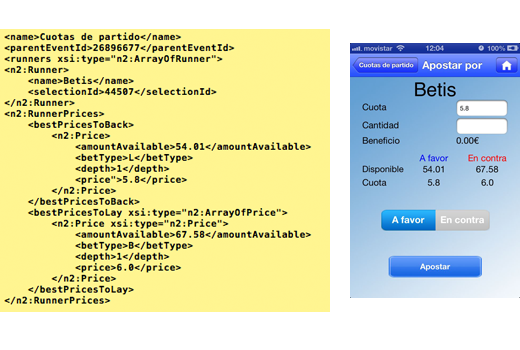
\includegraphics[width=0.8\textwidth]{./images/tabla_detail.png}
  \caption{Vista de tabla detallada del final de la jerarquía }
  \label{fig:detail-table-view}
\end{figure} 

\subsection{Arquitectura de la aplicación}	
   
   La aplicación esta formada principalmente por un conjunto de controladores de vista más un módulo encargado de comunicarse con el API de Betfair. Como hemos visto anteriormente, hemos hecho uso de las herramientas del SDK más adecuadas para navegar por la estructura de datos de Betfair. Para ello hemos creado diferentes controladores de vista para poder ofrecer al usuario la mejor vista para la representación de los datos en cada caso de uso.%\fixme{Fíjate que ésta es una decisión de diseño que aún no has explicado.}
   
   %\begin{figure} [h]
     %\centering
     %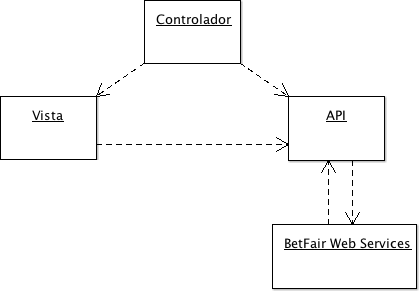
\includegraphics[width=0.8\textwidth]{./images/modelo1.png}
     %\caption{Esquema modelo vista controlador }
     %\label{fig:esquema-MVC}
   %\end{figure}
   
    %En la figura \ref{fig:esquema-MVC} podemos ver un esquema del modelo Vista Controlador usado. % \fxnote{de la arquitectura?}.
     %Los controladores de vista se encargan de recoger los eventos de la aplicación, principalmente \emph{inputs} del usuario. % \fxnote{eventos?}. 
     %En el caso de que el input involucre datos de Betfair, el controlador envía los datos necesarios para que el módulo de comunicación obtenga la respuesta por parte del API de Betfair. 
    
\subsubsection{Controlador principal}

 Es la clase principal de la aplicación. Es la encargada de iniciar el controlador de vista que será encargado de recoger los eventos del usuario, así como la gestión de memoria y la gestión de los eventos del sistema.
 
\subsubsection{Controlador de menú principal (RootViewController)}
 Es la encargada de mostrar las opciones principales del programa y recoger los inputs del usuario para lanzar el controlador adecuado a la elección del usuario. También se encarga de gestionar el inicio de sesión del usuario para los servicios web de Betfair. Para ello hace uso del servicio \emph{login} de Betfair a través de la clase de comunicación llamada API.
 
 \subsubsection{Controlador de perfil de usuario (ViewProfileController)}
 Muestra al usuario una lista con toda la información registrada en su perfil de Betfair, tales como el nombre de usuario, información de contacto y límite de apuestas diaría. Hace uso del servicio de Betfair \emph{ViewProfile}  a través de la clase API del modelo de la aplicación.
 
\subsubsection{Controlador de tipos de eventos (EventsTypeController)}
 Muestra al usuario una lista con todos los tipos de eventos activos por los que se puede apostar dentro de Betfair. En un futuro se podrá gestionar por fecha de finalización, orden alfabético o búsqueda directa de eventos. Una vez seleccionado el evento deseado, se lanza el controlador de eventos y mercados con la información relativa al evento previamente seleccionado. Hace uso del servicio de Betfair \emph{GetActiveEventsTypes}  a través de la clase API del modelo de la aplicación.
 
\subsubsection{Controlador de eventos y mercados (EventsAndMarketsController)}

 Es la clase encargada de mostrar de forma jerárquica los subeventos y mercados relacionados con un evento seleccionado previamente en el controlador de eventos. Igualmente se podrá gestionar por fecha de finalización, orden alfabético o búsqueda directa de eventos. En caso de ser seleccionado un evento, se le mostrará los mercados y subeventos relacionados con los mismos. Si se selecciona un mercado se procederá a lanzar el controlador de información de mercado. Para ello recaba la información obtenida a través del servicio web \emph{GetEvents} de Betfair.
 
\subsubsection{Controlador de información de mercado (MarketInfoController)}

 Es el responsable de gestionar toda la información relevante al mercado en cuestión. Gestionará el estado del mercado y sus propiedades obteniendo todo lo necesario del portal de Betfair a través del API de sus servicios web haciendo uso de las llamadas del API:
 
  \begin{itemize}
	\item \emph{GetMarket}: obtiene todos los parámetros acerca del mercado.
	\item \emph{GetMarketPrices}: obtiene todos los precios actuales del mercado en cuestión.
\end{itemize}

\subsubsection{Controlador de apuesta por un mercado (PutBetController)}
 Gestiona todos los datos necesarios e introducidos por el usuarios para realizar una apuesta y enviarla a Betfair. El método usado para enviar la apuesta a Betfair a través de la clase interfaz de comunicación es \emph{PlaceBets}.

\subsubsection{Controlador de las categorías de Mis Apuestas (MyBetsCategoryController)}
 Es la clase encargada de gestionar las apuestas ya realizadas en Betfair y que siguen activas. Las clasifica por categorías de mercado. Recoge la información como resultado de las llamadas a los siguientes servicios web de Betfair:
  \begin{itemize}
	\item \emph{GetMarket}: obtiene todos los parámetros acerca del mercado de una apuesta en cuestión.
	\item \emph{GetCurrentBets}: obtiene todas las apuestas realizadas por el usuario del servicios Betfair.
\end{itemize}
 
\subsubsection{Controlador de Mis Apuestas (MyBetsController)}
 Esta clase se encarga de gestionar las apuestas realizadas por el usuario dentro de una categoría determinada. En ella se muestra resumidamente el nombre de la apuesta en cuestión, la cuota apostada y la cuota actualizada en ese momento. 

\subsubsection{Controlador de detalles de una apuesta (MyBetDetailsController)}
 Se encarga de gestionar los detalles más relevantes sobre una apuesta determinada: parámetros, \emph{stake}, apuesta a favor o en contra relacionadas con la presentada\ldots También incluye información completa del mercado actual referente al mercado de la apuesta y el \emph{trading} acerca de la misma.
 
 \subsubsection{Controlador de propiedades de una apuesta (MyBetsProperties)}
 Se encarga de mostrar al usuario todos los detalles asociados a una apuesta determinada. 

\subsubsection{Controlador de \emph{trading} (TradingController)}
  Se encarga de asesorar al usuario sobre realizar el método \emph{trading} sobre una apuesta ya realizada. 
  
\subsubsection{API: Interfaz a Betfair}
 Esta clase se encarga de gestionar las comunicaciones con los servidores de Betfair. Envía las peticiones a los servicios web de Betfair y se encarga de realizar la decodificación de la respuesta a dichas peticiones en un formato adecuado para la aplicación.

\subsubsection{Controlador Parser (ParserXML)}
 Es la clase encargada de estructurar los datos de envío o recepción del servicio web a una estructura de datos adecuada para la aplicación y para la comunicación con Betfair.

\section{Diagrama de Estructura UML}
 En la figura \ref{fig:estructura} podemos ver el diagrama de la estructura del proyecto. Observamos que el núcleo principal de esta aplicación es la clase ``API''. Como bien hemos descrito, es la encargada de comunicarse con el servidor de Betfair tanto para enviar las peticiones como de procesar las respuestas. Esta clase necesita un \emph{parser} de XML para procesar los datos tantos del mensaje de petición de servicio como del mensaje de respuesta. De esta tarea se encarga la clase ``ParserXML''.
 
  Las clases que rodean a API son todos los controladores de vista de la aplicación. Son los que reciben las peticiones de la vista y, según el caso, hacer uso de un servicio concreto de Betfair a través de la clase ``API''. ``RootViewController'' es la clase a la que el sistema le otorga el control una vez se ha lanzado la aplicación. Su principal función es procesar el menú principal.

 \begin{figure}[h!]
    \centering
       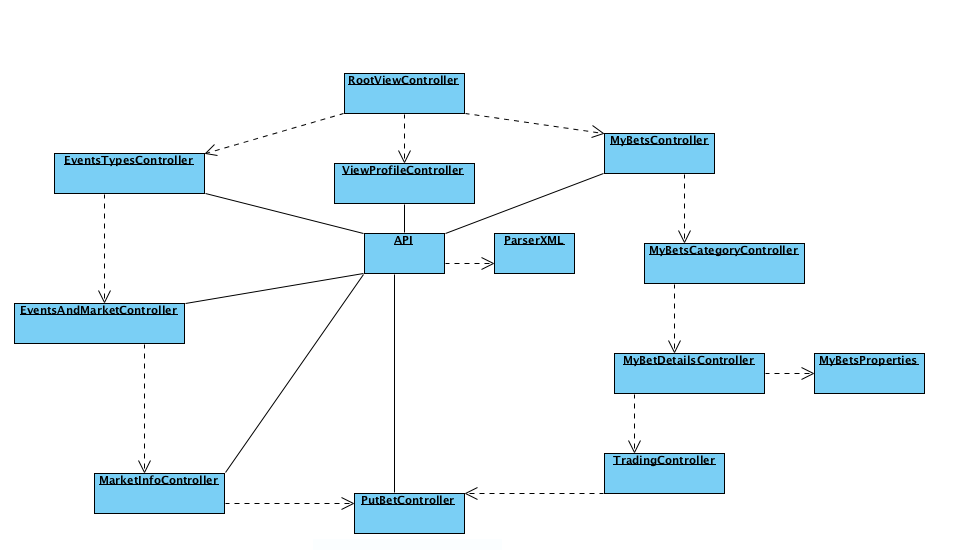
\includegraphics[width=0.95\linewidth]{./images/UML_Diagram.png}
     \caption{Diagrama de estructura UML}
   \label{fig:estructura}
\end{figure}

%%% Local Variables: 
%%% mode: latex
%%% TeX-master: "tfc-betfair-ios"
%%% TeX-PDF-mode: t
%%% ispell-local-dictionary: "castellano"
%%% End: 
